% =============================================================================
% Section 10 — Wire Protocol (TCP Framing)
% =============================================================================
\section{Wire Protocol: TCP Framing}
\label{sec:wire}

Both the gossip protocol and the client protocol transmit JSON-encoded payloads
over TCP using a shared length-type-payload framing layer implemented in
\pkg{wire}.

\subsection{Frame Format}

\begin{definition}[Wire frame]
A \emph{wire frame} is a contiguous byte sequence with the following layout:
\begin{center}
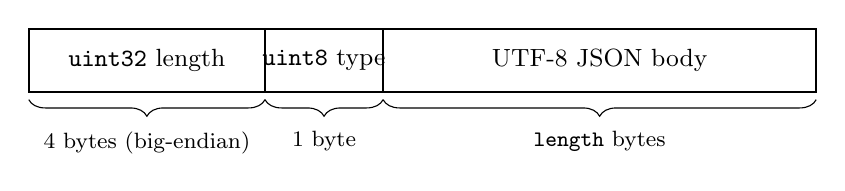
\begin{tikzpicture}[font=\small]
  \draw[thick] (0,0) rectangle (3, 0.8);
  \draw[thick] (3,0) rectangle (4.5, 0.8);
  \draw[thick] (4.5,0) rectangle (10, 0.8);

  \node at (1.5, 0.4) {\texttt{uint32} length};
  \node at (3.75, 0.4) {\texttt{uint8} type};
  \node at (7.25, 0.4) {UTF-8 JSON body};

  \draw[decorate, decoration={brace, amplitude=6pt, mirror}]
    (0, -0.1) -- (3, -0.1)
    node[midway, below=8pt, font=\footnotesize] {4 bytes (big-endian)};
  \draw[decorate, decoration={brace, amplitude=6pt, mirror}]
    (3, -0.1) -- (4.5, -0.1)
    node[midway, below=8pt, font=\footnotesize] {1 byte};
  \draw[decorate, decoration={brace, amplitude=6pt, mirror}]
    (4.5, -0.1) -- (10, -0.1)
    node[midway, below=8pt, font=\footnotesize] {\texttt{length} bytes};
\end{tikzpicture}
\end{center}
\begin{itemize}[leftmargin=1.5em]
  \item \textbf{length} (\texttt{uint32BE}): byte length of the JSON body only.
        The 5-byte header is not included in this count.
  \item \textbf{type} (\texttt{uint8}): message type identifier
        (from \texttt{GossipMessageType} or \texttt{ClientMessageType}).
  \item \textbf{body}: compact UTF-8 JSON.
\end{itemize}
\end{definition}

The total frame size is $5 + \mathit{length}$ bytes. The maximum permitted
body size is \texttt{limits.maxMessageBytes} (default: 10\,MiB).

\subsection{Message Type Constants}

\begin{table}[H]
\centering
\caption{Gossip and client protocol message type bytes.}
\label{tab:msg-types}
\begin{tabular}{@{}llll@{}}
\toprule
\multicolumn{2}{c}{\textbf{Gossip Protocol (port 7000)}} &
\multicolumn{2}{c}{\textbf{Client Protocol (port 7001)}} \\
\cmidrule(r){1-2}\cmidrule(l){3-4}
\textbf{Type} & \textbf{Byte} & \textbf{Type} & \textbf{Byte} \\
\midrule
\msg{HELLO}          & \texttt{0x01} & \msg{AUTH\_CHALLENGE}   & \texttt{0x10} \\
\msg{HELLO\_ACK}     & \texttt{0x02} & \msg{AUTH\_RESPONSE}    & \texttt{0x11} \\
\msg{HELLO\_CONFIRM} & \texttt{0x03} & \msg{AUTH\_ACK}         & \texttt{0x12} \\
\msg{PING}           & \texttt{0x04} & \msg{GET\_REQUEST}      & \texttt{0x20} \\
\msg{PONG}           & \texttt{0x05} & \msg{PUT\_REQUEST}      & \texttt{0x21} \\
\msg{DIGEST}         & \texttt{0x06} & \msg{DELETE\_REQUEST}   & \texttt{0x22} \\
\msg{REQUEST}        & \texttt{0x07} & \msg{KEYS\_REQUEST}     & \texttt{0x23} \\
\msg{MUTATIONS}      & \texttt{0x08} & \msg{ENTRIES\_REQUEST}  & \texttt{0x24} \\
\msg{ACK}            & \texttt{0x09} & \msg{GET\_RESPONSE}     & \texttt{0x30} \\
\msg{ERROR}          & \texttt{0x0a} & \msg{PUT\_RESPONSE}     & \texttt{0x31} \\
                     &               & \msg{DELETE\_RESPONSE}  & \texttt{0x32} \\
                     &               & \msg{KEYS\_RESPONSE}    & \texttt{0x33} \\
                     &               & \msg{ENTRIES\_RESPONSE} & \texttt{0x34} \\
                     &               & \msg{ERROR}             & \texttt{0x09} \\
\bottomrule
\end{tabular}
\end{table}

\subsection{Stream Decoder}

TCP is a byte-stream transport; a single \texttt{data} event may carry part of
a frame, a complete frame, or multiple frames. The \texttt{FrameDecoder} class
in \pkg{wire} maintains a reassembly buffer and emits complete frames:

\begin{enumerate}[leftmargin=1.5em]
  \item Incoming chunks are appended to an internal \texttt{Buffer}.
  \item The decoder checks whether the buffer contains at least 5 bytes (the
        header).
  \item If yes, it reads \texttt{length} from bytes 0--3 and \texttt{type}
        from byte 4.
  \item If \texttt{length} bytes of body are available (i.e., buffer length
        $\geq 5 + \mathit{length}$), the frame is extracted and emitted.
  \item If \texttt{length} exceeds \texttt{maxMessageBytes}, an error is emitted
        and the connection is closed, preventing OOM from a malformed or
        malicious message.
  \item The consumed bytes are removed from the buffer; the process repeats
        for any remaining data.
\end{enumerate}

This stateful push-based decoder correctly handles all TCP segmentation
scenarios and is tested with single-byte push streams.

\subsection{Encoding}

Frame encoding is straightforward:

\begin{lstlisting}[caption={Frame encoder (TypeScript).}]
export function encodeFrame(type: number, payload: unknown): Buffer {
  const body = Buffer.from(JSON.stringify(payload), "utf8");
  const frame = Buffer.allocUnsafe(5 + body.byteLength);
  frame.writeUInt32BE(body.byteLength, 0);
  frame.writeUInt8(type, 4);
  body.copy(frame, 5);
  return frame;
}
\end{lstlisting}

\subsection{DoS Considerations}

The \texttt{maxMessageBytes} limit defends against memory exhaustion by a peer
sending an oversized message. A frame with a \texttt{length} field exceeding
this limit triggers an immediate connection close without attempting to buffer
the body. This is the primary DoS surface in the current protocol; future
versions may add per-connection rate limiting and total in-flight byte limits.
